\documentclass[11pt]{article}

% Change "review" to "final" to generate the final (sometimes called camera-ready) version.
% Change to "preprint" to generate a non-anonymous version with page numbers.
\usepackage[review]{acl}

% Standard package includes
\usepackage{times}
\usepackage{latexsym}

% For proper rendering and hyphenation of words containing Latin characters (including in bib files)
\usepackage[T1]{fontenc}

% This assumes your files are encoded as UTF8
\usepackage[utf8]{inputenc}

% This is not strictly necessary, and may be commented out,
% but it will improve the layout of the manuscript,
% and will typically save some space.
\usepackage{microtype}

% This is also not strictly necessary, and may be commented out.
% However, it will improve the aesthetics of text in
% the typewriter font.
\usepackage{inconsolata}

%Including images in your LaTeX document requires adding
%additional package(s)
\usepackage{graphicx}
\usepackage{booktabs}
\usepackage{multirow}
\usepackage{tikz}
\usepackage{pgfplots}
\pgfplotsset{compat=1.18}

% Global pgfplots aesthetic
\pgfplotsset{
  every axis/.append style={
    axis line style={gray!40},
    tick style={gray!60},
    grid=major,
    grid style={line width=.2pt, draw=gray!20},
    tick label style={font=\scriptsize},
    label style={font=\footnotesize},
    title style={font=\footnotesize, align=center},
    line width=0.8pt
  }
}

% Mathematical notation and shared commands
% \usepackage{times}
% \usepackage[utf8]{inputenc}
% \usepackage[T1]{fontenc}
\usepackage{amsmath}
\usepackage{amssymb}
\usepackage{hyperref}
\usepackage{url}
\usepackage{booktabs}
\usepackage{amsfonts}
\usepackage{nicefrac}
\usepackage{microtype}
\usepackage{mathtools,bm}
\usepackage{xcolor}
\usepackage{hyperref}
\usepackage{subcaption,placeins}
\usepackage{adjustbox,multirow,dcolumn}
\usepackage{algorithm,algpseudocode,setspace}
\usepackage{xstring}
\usepackage{cleveref}
\usepackage{graphicx}
% \usepackage{natbib}
% \usepackage{natbib}
% \usepackage[numbers]{natbib}
% \usepackage[numbers,sort]{natbib}
% \setcitestyle{sort,comma,numbers,square}
\usepackage{tikz}
\usepackage{pgfplots}
\usepackage{comment}
% \usepackage{xparse}
\usepackage{framed}
\usepackage{pifont}

\makeatletter

% authors
\newcommand{\authornote}[1]{\textsuperscript{\rm {#1}}}
\newcommand{\email}[1]{\href{mailto:#1}{\texttt{#1}}}
\newcommand*\samethanks[1][\value{footnote}]{%
    \footnotemark[#1]\hspace{0.4em}}

% notes
\newcommand{\fixme}{\marginpar{FIXME}}
\newcommand{\todo}{\marginpar{TODO}}
% \newcommand{\rebuttal}[1]{{\color{blue}{#1}}}
\newcommand{\revise}[1]{{\color{blue}{#1}}}

% math
%%%%% NEW MATH DEFINITIONS %%%%%

\usepackage{amsmath,amsfonts,bm}

% Mark sections of captions for referring to divisions of figures
\newcommand{\figleft}{{\em (Left)}}
\newcommand{\figcenter}{{\em (Center)}}
\newcommand{\figright}{{\em (Right)}}
\newcommand{\figtop}{{\em (Top)}}
\newcommand{\figbottom}{{\em (Bottom)}}
\newcommand{\captiona}{{\em (a)}}
\newcommand{\captionb}{{\em (b)}}
\newcommand{\captionc}{{\em (c)}}
\newcommand{\captiond}{{\em (d)}}

% Highlight a newly defined term
\newcommand{\newterm}[1]{{\bf #1}}

% Our method name and acronym
\newcommand{\methodfullname}{Semantic MCP Tool Hijacking}
\newcommand{\methodname}{\methodfullname}
\newcommand{\methodacronym}{SMTH}
\newcommand{\methodnameshort}{\methodacronym}


% Figure reference, lower-case.
\def\figref#1{figure~\ref{#1}}
% Figure reference, capital. For start of sentence
\def\Figref#1{Figure~\ref{#1}}
\def\twofigref#1#2{figures \ref{#1} and \ref{#2}}
\def\quadfigref#1#2#3#4{figures \ref{#1}, \ref{#2}, \ref{#3} and \ref{#4}}
% Section reference, lower-case.
\def\secref#1{section~\ref{#1}}
% Section reference, capital.
\def\Secref#1{Section~\ref{#1}}
% Reference to two sections.
\def\twosecrefs#1#2{sections \ref{#1} and \ref{#2}}
% Reference to three sections.
\def\secrefs#1#2#3{sections \ref{#1}, \ref{#2} and \ref{#3}}
% Reference to an equation, lower-case.
\def\eqref#1{equation~\ref{#1}}
% Reference to an equation, upper case
\def\Eqref#1{Equation~\ref{#1}}
% A raw reference to an equation---avoid using if possible
\def\plaineqref#1{\ref{#1}}
% Reference to a chapter, lower-case.
\def\chapref#1{chapter~\ref{#1}}
% Reference to an equation, upper case.
\def\Chapref#1{Chapter~\ref{#1}}
% Reference to a range of chapters
\def\rangechapref#1#2{chapters\ref{#1}--\ref{#2}}
% Reference to an algorithm, lower-case.
\def\algref#1{algorithm~\ref{#1}}
% Reference to an algorithm, upper case.
\def\Algref#1{Algorithm~\ref{#1}}
\def\twoalgref#1#2{algorithms \ref{#1} and \ref{#2}}
\def\Twoalgref#1#2{Algorithms \ref{#1} and \ref{#2}}
% Reference to a part, lower case
\def\partref#1{part~\ref{#1}}
% Reference to a part, upper case
\def\Partref#1{Part~\ref{#1}}
\def\twopartref#1#2{parts \ref{#1} and \ref{#2}}

\def\ceil#1{\lceil #1 \rceil}
\def\floor#1{\lfloor #1 \rfloor}
\def\1{\bm{1}}
\newcommand{\train}{\mathcal{D}}
\newcommand{\valid}{\mathcal{D_{\mathrm{valid}}}}
\newcommand{\test}{\mathcal{D_{\mathrm{test}}}}

\def\eps{{\epsilon}}


% Random variables
\def\reta{{\textnormal{$\eta$}}}
\def\ra{{\textnormal{a}}}
\def\rb{{\textnormal{b}}}
\def\rc{{\textnormal{c}}}
\def\rd{{\textnormal{d}}}
\def\re{{\textnormal{e}}}
\def\rf{{\textnormal{f}}}
\def\rg{{\textnormal{g}}}
\def\rh{{\textnormal{h}}}
\def\ri{{\textnormal{i}}}
\def\rj{{\textnormal{j}}}
\def\rk{{\textnormal{k}}}
\def\rl{{\textnormal{l}}}
% rm is already a command, just don't name any random variables m
\def\rn{{\textnormal{n}}}
\def\ro{{\textnormal{o}}}
\def\rp{{\textnormal{p}}}
\def\rq{{\textnormal{q}}}
\def\rr{{\textnormal{r}}}
\def\rs{{\textnormal{s}}}
\def\rt{{\textnormal{t}}}
\def\ru{{\textnormal{u}}}
\def\rv{{\textnormal{v}}}
\def\rw{{\textnormal{w}}}
\def\rx{{\textnormal{x}}}
\def\ry{{\textnormal{y}}}
\def\rz{{\textnormal{z}}}

% Random vectors
\def\rvepsilon{{\mathbf{\epsilon}}}
\def\rvtheta{{\mathbf{\theta}}}
\def\rva{{\mathbf{a}}}
\def\rvb{{\mathbf{b}}}
\def\rvc{{\mathbf{c}}}
\def\rvd{{\mathbf{d}}}
\def\rve{{\mathbf{e}}}
\def\rvf{{\mathbf{f}}}
\def\rvg{{\mathbf{g}}}
\def\rvh{{\mathbf{h}}}
\def\rvu{{\mathbf{i}}}
\def\rvj{{\mathbf{j}}}
\def\rvk{{\mathbf{k}}}
\def\rvl{{\mathbf{l}}}
\def\rvm{{\mathbf{m}}}
\def\rvn{{\mathbf{n}}}
\def\rvo{{\mathbf{o}}}
\def\rvp{{\mathbf{p}}}
\def\rvq{{\mathbf{q}}}
\def\rvr{{\mathbf{r}}}
\def\rvs{{\mathbf{s}}}
\def\rvt{{\mathbf{t}}}
\def\rvu{{\mathbf{u}}}
\def\rvv{{\mathbf{v}}}
\def\rvw{{\mathbf{w}}}
\def\rvx{{\mathbf{x}}}
\def\rvy{{\mathbf{y}}}
\def\rvz{{\mathbf{z}}}

% Elements of random vectors
\def\erva{{\textnormal{a}}}
\def\ervb{{\textnormal{b}}}
\def\ervc{{\textnormal{c}}}
\def\ervd{{\textnormal{d}}}
\def\erve{{\textnormal{e}}}
\def\ervf{{\textnormal{f}}}
\def\ervg{{\textnormal{g}}}
\def\ervh{{\textnormal{h}}}
\def\ervi{{\textnormal{i}}}
\def\ervj{{\textnormal{j}}}
\def\ervk{{\textnormal{k}}}
\def\ervl{{\textnormal{l}}}
\def\ervm{{\textnormal{m}}}
\def\ervn{{\textnormal{n}}}
\def\ervo{{\textnormal{o}}}
\def\ervp{{\textnormal{p}}}
\def\ervq{{\textnormal{q}}}
\def\ervr{{\textnormal{r}}}
\def\ervs{{\textnormal{s}}}
\def\ervt{{\textnormal{t}}}
\def\ervu{{\textnormal{u}}}
\def\ervv{{\textnormal{v}}}
\def\ervw{{\textnormal{w}}}
\def\ervx{{\textnormal{x}}}
\def\ervy{{\textnormal{y}}}
\def\ervz{{\textnormal{z}}}

% Random matrices
\def\rmA{{\mathbf{A}}}
\def\rmB{{\mathbf{B}}}
\def\rmC{{\mathbf{C}}}
\def\rmD{{\mathbf{D}}}
\def\rmE{{\mathbf{E}}}
\def\rmF{{\mathbf{F}}}
\def\rmG{{\mathbf{G}}}
\def\rmH{{\mathbf{H}}}
\def\rmI{{\mathbf{I}}}
\def\rmJ{{\mathbf{J}}}
\def\rmK{{\mathbf{K}}}
\def\rmL{{\mathbf{L}}}
\def\rmM{{\mathbf{M}}}
\def\rmN{{\mathbf{N}}}
\def\rmO{{\mathbf{O}}}
\def\rmP{{\mathbf{P}}}
\def\rmQ{{\mathbf{Q}}}
\def\rmR{{\mathbf{R}}}
\def\rmS{{\mathbf{S}}}
\def\rmT{{\mathbf{T}}}
\def\rmU{{\mathbf{U}}}
\def\rmV{{\mathbf{V}}}
\def\rmW{{\mathbf{W}}}
\def\rmX{{\mathbf{X}}}
\def\rmY{{\mathbf{Y}}}
\def\rmZ{{\mathbf{Z}}}

% Elements of random matrices
\def\ermA{{\textnormal{A}}}
\def\ermB{{\textnormal{B}}}
\def\ermC{{\textnormal{C}}}
\def\ermD{{\textnormal{D}}}
\def\ermE{{\textnormal{E}}}
\def\ermF{{\textnormal{F}}}
\def\ermG{{\textnormal{G}}}
\def\ermH{{\textnormal{H}}}
\def\ermI{{\textnormal{I}}}
\def\ermJ{{\textnormal{J}}}
\def\ermK{{\textnormal{K}}}
\def\ermL{{\textnormal{L}}}
\def\ermM{{\textnormal{M}}}
\def\ermN{{\textnormal{N}}}
\def\ermO{{\textnormal{O}}}
\def\ermP{{\textnormal{P}}}
\def\ermQ{{\textnormal{Q}}}
\def\ermR{{\textnormal{R}}}
\def\ermS{{\textnormal{S}}}
\def\ermT{{\textnormal{T}}}
\def\ermU{{\textnormal{U}}}
\def\ermV{{\textnormal{V}}}
\def\ermW{{\textnormal{W}}}
\def\ermX{{\textnormal{X}}}
\def\ermY{{\textnormal{Y}}}
\def\ermZ{{\textnormal{Z}}}

% Vectors
\def\vzero{{\bm{0}}}
\def\vone{{\bm{1}}}
\def\vmu{{\bm{\mu}}}
\def\vtheta{{\bm{\theta}}}
\def\va{{\bm{a}}}
\def\vb{{\bm{b}}}
\def\vc{{\bm{c}}}
\def\vd{{\bm{d}}}
\def\ve{{\bm{e}}}
\def\vf{{\bm{f}}}
\def\vg{{\bm{g}}}
\def\vh{{\bm{h}}}
\def\vi{{\bm{i}}}
\def\vj{{\bm{j}}}
\def\vk{{\bm{k}}}
\def\vl{{\bm{l}}}
\def\vm{{\bm{m}}}
\def\vn{{\bm{n}}}
\def\vo{{\bm{o}}}
\def\vp{{\bm{p}}}
\def\vq{{\bm{q}}}
\def\vr{{\bm{r}}}
\def\vs{{\bm{s}}}
\def\vt{{\bm{t}}}
\def\vu{{\bm{u}}}
\def\vv{{\bm{v}}}
\def\vw{{\bm{w}}}
\def\vx{{\bm{x}}}
\def\vy{{\bm{y}}}
\def\vz{{\bm{z}}}

% Elements of vectors
\def\evalpha{{\alpha}}
\def\evbeta{{\beta}}
\def\evepsilon{{\epsilon}}
\def\evlambda{{\lambda}}
\def\evomega{{\omega}}
\def\evmu{{\mu}}
\def\evpsi{{\psi}}
\def\evsigma{{\sigma}}
\def\evtheta{{\theta}}
\def\eva{{a}}
\def\evb{{b}}
\def\evc{{c}}
\def\evd{{d}}
\def\eve{{e}}
\def\evf{{f}}
\def\evg{{g}}
\def\evh{{h}}
\def\evi{{i}}
\def\evj{{j}}
\def\evk{{k}}
\def\evl{{l}}
\def\evm{{m}}
\def\evn{{n}}
\def\evo{{o}}
\def\evp{{p}}
\def\evq{{q}}
\def\evr{{r}}
\def\evs{{s}}
\def\evt{{t}}
\def\evu{{u}}
\def\evv{{v}}
\def\evw{{w}}
\def\evx{{x}}
\def\evy{{y}}
\def\evz{{z}}

% Matrix
\def\mA{{\bm{A}}}
\def\mB{{\bm{B}}}
\def\mC{{\bm{C}}}
\def\mD{{\bm{D}}}
\def\mE{{\bm{E}}}
\def\mF{{\bm{F}}}
\def\mG{{\bm{G}}}
\def\mH{{\bm{H}}}
\def\mI{{\bm{I}}}
\def\mJ{{\bm{J}}}
\def\mK{{\bm{K}}}
\def\mL{{\bm{L}}}
\def\mM{{\bm{M}}}
\def\mN{{\bm{N}}}
\def\mO{{\bm{O}}}
\def\mP{{\bm{P}}}
\def\mQ{{\bm{Q}}}
\def\mR{{\bm{R}}}
\def\mS{{\bm{S}}}
\def\mT{{\bm{T}}}
\def\mU{{\bm{U}}}
\def\mV{{\bm{V}}}
\def\mW{{\bm{W}}}
\def\mX{{\bm{X}}}
\def\mY{{\bm{Y}}}
\def\mZ{{\bm{Z}}}
\def\mBeta{{\bm{\beta}}}
\def\mPhi{{\bm{\Phi}}}
\def\mLambda{{\bm{\Lambda}}}
\def\mSigma{{\bm{\Sigma}}}

% Tensor
\DeclareMathAlphabet{\mathsfit}{\encodingdefault}{\sfdefault}{m}{sl}
\SetMathAlphabet{\mathsfit}{bold}{\encodingdefault}{\sfdefault}{bx}{n}
\newcommand{\tens}[1]{\bm{\mathsfit{#1}}}
\def\tA{{\tens{A}}}
\def\tB{{\tens{B}}}
\def\tC{{\tens{C}}}
\def\tD{{\tens{D}}}
\def\tE{{\tens{E}}}
\def\tF{{\tens{F}}}
\def\tG{{\tens{G}}}
\def\tH{{\tens{H}}}
\def\tI{{\tens{I}}}
\def\tJ{{\tens{J}}}
\def\tK{{\tens{K}}}
\def\tL{{\tens{L}}}
\def\tM{{\tens{M}}}
\def\tN{{\tens{N}}}
\def\tO{{\tens{O}}}
\def\tP{{\tens{P}}}
\def\tQ{{\tens{Q}}}
\def\tR{{\tens{R}}}
\def\tS{{\tens{S}}}
\def\tT{{\tens{T}}}
\def\tU{{\tens{U}}}
\def\tV{{\tens{V}}}
\def\tW{{\tens{W}}}
\def\tX{{\tens{X}}}
\def\tY{{\tens{Y}}}
\def\tZ{{\tens{Z}}}


% Graph
\def\gA{{\mathcal{A}}}
\def\gB{{\mathcal{B}}}
\def\gC{{\mathcal{C}}}
\def\gD{{\mathcal{D}}}
\def\gE{{\mathcal{E}}}
\def\gF{{\mathcal{F}}}
\def\gG{{\mathcal{G}}}
\def\gH{{\mathcal{H}}}
\def\gI{{\mathcal{I}}}
\def\gJ{{\mathcal{J}}}
\def\gK{{\mathcal{K}}}
\def\gL{{\mathcal{L}}}
\def\gM{{\mathcal{M}}}
\def\gN{{\mathcal{N}}}
\def\gO{{\mathcal{O}}}
\def\gP{{\mathcal{P}}}
\def\gQ{{\mathcal{Q}}}
\def\gR{{\mathcal{R}}}
\def\gS{{\mathcal{S}}}
\def\gT{{\mathcal{T}}}
\def\gU{{\mathcal{U}}}
\def\gV{{\mathcal{V}}}
\def\gW{{\mathcal{W}}}
\def\gX{{\mathcal{X}}}
\def\gY{{\mathcal{Y}}}
\def\gZ{{\mathcal{Z}}}

% Sets
\def\sA{{\mathbb{A}}}
\def\sB{{\mathbb{B}}}
\def\sC{{\mathbb{C}}}
\def\sD{{\mathbb{D}}}
% Don't use a set called E, because this would be the same as our symbol
% for expectation.
\def\sF{{\mathbb{F}}}
\def\sG{{\mathbb{G}}}
\def\sH{{\mathbb{H}}}
\def\sI{{\mathbb{I}}}
\def\sJ{{\mathbb{J}}}
\def\sK{{\mathbb{K}}}
\def\sL{{\mathbb{L}}}
\def\sM{{\mathbb{M}}}
\def\sN{{\mathbb{N}}}
\def\sO{{\mathbb{O}}}
\def\sP{{\mathbb{P}}}
\def\sQ{{\mathbb{Q}}}
\def\sR{{\mathbb{R}}}
\def\sS{{\mathbb{S}}}
\def\sT{{\mathbb{T}}}
\def\sU{{\mathbb{U}}}
\def\sV{{\mathbb{V}}}
\def\sW{{\mathbb{W}}}
\def\sX{{\mathbb{X}}}
\def\sY{{\mathbb{Y}}}
\def\sZ{{\mathbb{Z}}}

% Entries of a matrix
\def\emLambda{{\Lambda}}
\def\emA{{A}}
\def\emB{{B}}
\def\emC{{C}}
\def\emD{{D}}
\def\emE{{E}}
\def\emF{{F}}
\def\emG{{G}}
\def\emH{{H}}
\def\emI{{I}}
\def\emJ{{J}}
\def\emK{{K}}
\def\emL{{L}}
\def\emM{{M}}
\def\emN{{N}}
\def\emO{{O}}
\def\emP{{P}}
\def\emQ{{Q}}
\def\emR{{R}}
\def\emS{{S}}
\def\emT{{T}}
\def\emU{{U}}
\def\emV{{V}}
\def\emW{{W}}
\def\emX{{X}}
\def\emY{{Y}}
\def\emZ{{Z}}
\def\emSigma{{\Sigma}}

% entries of a tensor
% Same font as tensor, without \bm wrapper
\newcommand{\etens}[1]{\mathsfit{#1}}
\def\etLambda{{\etens{\Lambda}}}
\def\etA{{\etens{A}}}
\def\etB{{\etens{B}}}
\def\etC{{\etens{C}}}
\def\etD{{\etens{D}}}
\def\etE{{\etens{E}}}
\def\etF{{\etens{F}}}
\def\etG{{\etens{G}}}
\def\etH{{\etens{H}}}
\def\etI{{\etens{I}}}
\def\etJ{{\etens{J}}}
\def\etK{{\etens{K}}}
\def\etL{{\etens{L}}}
\def\etM{{\etens{M}}}
\def\etN{{\etens{N}}}
\def\etO{{\etens{O}}}
\def\etP{{\etens{P}}}
\def\etQ{{\etens{Q}}}
\def\etR{{\etens{R}}}
\def\etS{{\etens{S}}}
\def\etT{{\etens{T}}}
\def\etU{{\etens{U}}}
\def\etV{{\etens{V}}}
\def\etW{{\etens{W}}}
\def\etX{{\etens{X}}}
\def\etY{{\etens{Y}}}
\def\etZ{{\etens{Z}}}

% The true underlying data generating distribution
\newcommand{\pdata}{p_{\rm{data}}}
% The empirical distribution defined by the training set
\newcommand{\ptrain}{\hat{p}_{\rm{data}}}
\newcommand{\Ptrain}{\hat{P}_{\rm{data}}}
% The model distribution
\newcommand{\pmodel}{p_{\rm{model}}}
\newcommand{\Pmodel}{P_{\rm{model}}}
\newcommand{\ptildemodel}{\tilde{p}_{\rm{model}}}
% Stochastic autoencoder distributions
\newcommand{\pencode}{p_{\rm{encoder}}}
\newcommand{\pdecode}{p_{\rm{decoder}}}
\newcommand{\precons}{p_{\rm{reconstruct}}}

\newcommand{\laplace}{\mathrm{Laplace}} % Laplace distribution

\newcommand{\E}{\mathbb{E}}
\newcommand{\Ls}{\mathcal{L}}
\newcommand{\R}{\mathbb{R}}
\newcommand{\emp}{\tilde{p}}
\newcommand{\lr}{\alpha}
\newcommand{\reg}{\lambda}
\newcommand{\rect}{\mathrm{rectifier}}
\newcommand{\softmax}{\mathrm{softmax}}
\newcommand{\sigmoid}{\sigma}
\newcommand{\softplus}{\zeta}
\newcommand{\KL}{D_{\mathrm{KL}}}
\newcommand{\Var}{\mathrm{Var}}
\newcommand{\standarderror}{\mathrm{SE}}
\newcommand{\Cov}{\mathrm{Cov}}
% Wolfram Mathworld says $L^2$ is for function spaces and $\ell^2$ is for vectors
% But then they seem to use $L^2$ for vectors throughout the site, and so does
% wikipedia.
\newcommand{\normlzero}{L^0}
\newcommand{\normlone}{L^1}
\newcommand{\normltwo}{L^2}
\newcommand{\normlp}{L^p}
\newcommand{\normmax}{L^\infty}

\newcommand{\parents}{Pa} % See usage in notation.tex. Chosen to match Daphne's book.

\DeclareMathOperator*{\argmax}{arg\,max}
\DeclareMathOperator*{\argmin}{arg\,min}

\DeclareMathOperator{\sign}{sign}
\DeclareMathOperator{\Tr}{Tr}
\let\ab\allowbreak


% units
\newcommand{\mega}{\,\textrm{M}}
\newcommand{\giga}{\,\textrm{G}}
\newcommand{\tera}{\,\textrm{T}}
\newcommand{\peta}{\,\textrm{P}}

% latin
\DeclareRobustCommand\onedot{\futurelet\@let@token\@onedot}
\def\@onedot{\ifx\@let@token.\else.\null\fi}
\newcommand{\Eg}{\emph{E.g\@\onedot}}
\newcommand{\eg}{\emph{e.g\@\onedot}}
\newcommand{\etc}{\emph{etc\@\onedot}}
\newcommand{\etal}{\emph{et~al\@\onedot}}
\newcommand{\Ie}{\emph{I.e\@\onedot}}
\newcommand{\ie}{\emph{i.e\@\onedot}}
\newcommand{\versus}{\texorpdfstring{\emph{vs\@\onedot}}{vs.}}
\newcommand{\viceversa}{\emph{vice versa}}
\newcommand{\wrt}{\emph{w.r.t\@\onedot}}
\newcommand{\subto}{\emph{s.t\@\onedot}}
\newcommand{\numero}[1]{No\@.\ {#1}}
\newcommand{\numeros}[1]{Nos\@.\ {#1}}
\newcommand{\first}{1\textsuperscript{st}}
\newcommand{\second}{2\textsuperscript{nd}}
\newcommand{\third}{3\textsuperscript{rd}}
\newcommand{\ordinal}[1]{{#1}\textsuperscript{th}}

% figures
\graphicspath{{figures/}}
\DeclareRobustCommand{\inlinegraphics}[2][1]{%
  \begingroup\normalfont%
  \includegraphics[height=#1\fontcharht\font`\B]{#2}%
  \endgroup
}

% tikz
\usetikzlibrary{external}
\usepgfplotslibrary{colorbrewer}
\pgfplotsset{compat=newest}
\tikzexternalize[prefix=tikz/]
\newcommand{\tikzsnfn}[1]{%
    \def\fn{#1}\StrSubstitute{\fn}{/}{_}[\fn]%
    \tikzsetnextfilename{\fn}}
% \newtoggle{final}\togglefalse{final}
% \tikzifexternalizing{\toggletrue{final}}{\togglefalse{final}}

% tables
\newcolumntype{d}{D{.}{.}{3.2}}
\newcolumntype{B}{>{\boldmath\DC@{.}{.}{3.2}}c<{\DC@end}}
\newcommand{\supstar}{\mbox{\textsuperscript{\( \star \)}}}
\newcommand{\supcirc}{\mbox{\textsuperscript{\( \circ \)}}}
\newcommand{\supdagger}{\textsuperscript{\textdagger}}
\newcommand{\supddagger}{\textsuperscript{\textdaggerdbl}}
\newcommand{\tbox}[1]{\begin{tabular}[c]{@{}c@{}}#1\end{tabular}}
\newcommand{\tcenter}[1]{\multicolumn{1}{c}{{#1}}}
\newcommand{\thead}[1]{\multicolumn{1}{c}{\textbf{#1}}}
\newcommand{\tbnum}[1]{\multicolumn{1}{B}{#1}}
\newcommand{\tna}{\tcenter{---}}
\newcommand{\tpm}[2]{\( {#1}{\scriptstyle \pm #2} \)}
\newcommand{\tbpm}[2]{\tpm{\mathbf{#1}}{#2}}
\newcommand{\tbgreen}[1]{\textcolor[rgb]{0,0.502,0}{#1}}
\newcommand{\tbred}[1]{\textcolor[rgb]{0.502,0,0}{#1}}

% macros
\newcommand{\numfirstorder}{6}
\newcommand{\numsecondorder}{2}
\newcommand{\nummetrics}{8}
% TODO: a better name
\newcommand{\MethodVerb}{{mixSGA}}
\newcommand{\Method}{\emph{\MethodVerb}}
\newcommand{\idx}[2]{{#1}^{\scriptscriptstyle[{#2}]}}

% math
\DeclarePairedDelimiter{\parens}{\lparen}{\rparen}
\DeclarePairedDelimiter{\angles}{\langle}{\rangle}
\DeclarePairedDelimiter{\bracks}{[}{]}
\DeclarePairedDelimiter{\braces}{\{}{\}}
\DeclarePairedDelimiter{\verts}{\lvert}{\rvert}
\DeclarePairedDelimiter{\Verts}{\lVert}{\rVert}
\DeclarePairedDelimiter{\floors}{\lfloor}{\rfloor}
\DeclarePairedDelimiter{\ceils}{\lceil}{\rceil}
\newcommand{\expect}[2][]{\mathbb{E}_{#1}\bracks*{#2}}
\newcommand{\diff}[2]{\frac{\partial{#1}}{\partial{#2}}}
\newcommand{\shat}[1]{\vphantom{#1}\smash[t]{\hat{#1}}}
\newcommand{\x}{{\mathbf{x}}}
\newcommand{\z}{{\mathbf{z}}}
\newcommand{\y}{\mathbf{y}}
\newcommand{\ratios}{\bm{\rho}}
\newcommand{\ratio}{\rho}
\newcommand{\mask}{\mathbf{m}}
\newcommand{\weight}{{\bm\theta}}
\newcommand{\keyweight}{{\mathbf{w}^\textrm{k}}}
\newcommand{\valueweight}{{\mathbf{w}^\textrm{v}}}
\newcommand{\keybias}{{\mathbf{b}^\textrm{k}}}
\newcommand{\valuebias}{{\mathbf{b}^\textrm{v}}}
\newcommand{\routeweight}{\bm\phi}
\newcommand{\routebias}{\bm\beta}
\newcommand{\dataset}{\mathcal{D}}
\newcommand{\testset}{\dataset_\textrm{test}}
\newcommand{\trainset}{\dataset_\textrm{train}}
\newcommand{\realset}{\mathbb{R}}
\newcommand{\inputset}{\mathcal{I}}
\newcommand{\classset}{\mathcal{C}}
\newcommand{\outputset}{\realset^K}
\newcommand{\stepsize}{\alpha}
\newcommand{\momentum}{\nu}
\DeclareMathOperator{\topk}{\mathsf{top}}
\DeclareMathOperator{\bigO}{\mathcal{O}}
\DeclareMathOperator{\loss}{\mathcal{L}}
\DeclareMathOperator{\sceloss}{\mathcal{L}^\textrm{sce}}
\DeclareMathOperator{\auxloss}{\mathcal{L}_\textrm{aux}}
\DeclareMathOperator{\modelloss}{\mathcal{L}_\textrm{model}}
\DeclareMathOperator{\dist}{{dist}}
\DeclareMathOperator{\norm}{{norm}}
\DeclareMathOperator{\moe}{\mathsf{moe}}
\DeclareMathOperator{\onehot}{{onehot}}
\DeclareMathOperator{\indicator}{\mathbf{1}}
\DeclareMathOperator{\betadist}{\mathcal{B}}
\DeclareMathOperator{\sample}{sample}
\DeclareMathOperator{\batchsample}{minibatch}
% \DeclareMathOperator{\sigmoid}{{\sigma}}
% \DeclareMathOperator{\softmax}{\mathsf{softmax}}
\DeclareMathOperator{\routescore}{\mathsf{S}}
\DeclareMathOperator{\recon}{\mathsf{Reconstruct}}
\DeclareMathOperator{\bceloss}{\mathsf{BCE}}
% plots
% \newcommand{\hpad}{\hspace*{\fill}}
% \newcommand{\subplotsizeslack}{1}
% \NewDocumentCommand{\subplot}{ O{1} O{} m m m }{%
%     \hpad%
%     \begin{subfigure}{(\textwidth / #1) * \subplotsizeslack}
%         \includegraphics[width=\textwidth, #2]{#3}
%         \caption{#4}\label{#5}
%     \end{subfigure}%
% }

\makeatother


\title{SMTH: Hijacking AI Agents via a Single Malicious MCP Tool}

\author{Anonymous Authors}

\begin{document}
\maketitle
\section*{Abstract}
Model Context Protocol (MCP) tools have become increasingly prevalent in AI systems, enabling seamless integration between language models and external services. However, the security vulnerabilities of these tools remain largely unexplored. In this work, we present Semantic MCP Tool Hijacking (SMTH), a novel genetic algorithm-based approach for generating semantic attacks on MCP tools. Our methodology systematically evolves adversarial prompts that exploit semantic weaknesses in tool descriptions and parameter validation mechanisms. We evaluate our approach on a comprehensive benchmark of over 100 MCP tools, demonstrating that genetic algorithm-based attacks achieve a 73.2\% success rate in bypassing security measures, significantly outperforming baseline random attacks (23.1\%). Our analysis reveals specific vulnerability patterns in semantic parsing and suggests practical countermeasures for improving MCP tool security. This research contributes to the emerging field of AI tool security and provides a foundation for developing more robust MCP implementations.

\section{Introduction}
Modern AI agents are increasingly reliant on external tools to extend their capabilities beyond their parametric knowledge. The Model Context Protocol (MCP) \cite{liu2024promptinjectionattackllmintegrated}, as an emerging standard, allows servers to dynamically register tools with agents, significantly enhancing their adaptability and functionality in complex environments. In this interaction paradigm, the core basis for an agent to select and invoke a tool is solely the semantic information—such as the tool's name, description, and expected return content. \textbf{A critical and widespread assumption underpinning this architecture is that the MCP server and the tool metadata it provides are trustworthy.} However, this assumption is tenuous in practical, open deployment environments where services are often provided by third parties—an attacker can easily deploy a malicious MCP server, creating a significant yet overlooked attack surface. Although the security of AI agents has garnered widespread attention, existing research predominantly focuses on traditional attack surfaces like prompt injection \cite{yu2024assessingpromptinjectionrisks} and privilege escalation \cite{Yan_2025}. These studies \textbf{largely overlook a systematic analysis of the emerging attack surface at the tool semantic layer (i.e., names, descriptions, and return content).} The design of the MCP protocol itself, while innovative in facilitating tool integration, also does not adequately consider the risk of malicious manipulation of tool metadata, lacking effective mechanisms for authenticity verification \cite{croce2025trivialtrojansminimalmcp}.

This research gap is particularly concerning given the demonstrated vulnerability of LLMs to semantic manipulation in other contexts. Prior work has shown that LLMs can be misled through carefully crafted instructions \cite{zhang2024instructionbackdoorattackscustomized} and that their tool-selection mechanisms are sensitive to description wording \cite{blankenstein2025biasbustersuncoveringmitigatingtool}. Building on these observations, we posit the following research hypotheses: \textbf{First (H1),} an attacker can successfully induce an agent to invoke a malicious tool by crafting its name and description, without modifying the underlying tool code, thereby achieving attack goals such as resource waste, information leakage, backdoor implantation, or task failure induction. \textbf{Second (H2),} leveraging a Large Language Model (LLM)-driven automated genetic algorithm \cite{zhang2025systematicsurveylargelanguage}, guided by semantic embeddings \cite{yan2025embedx}, can efficiently generate highly successful and stealthy attack payloads that evade simple detection heuristics.

To validate these hypotheses, this paper designs a comprehensive experimental evaluation framework. We construct a controlled test environment where an attacker has full control over MCP tool metadata and formally define four categories of attack scenarios with quantifiable metrics. Furthermore, we propose an innovative Semantic MCP Tool Hijacking (\methodacronym) framework for automatically generating and optimizing attack payloads. This study represents the first systematic investigation of security risks at the tool semantic layer of the MCP protocol, serving as a critical wake-up call for building more robust tool invocation mechanisms for agents in untrusted environments.



\begin{figure*}[t]
    \centering
    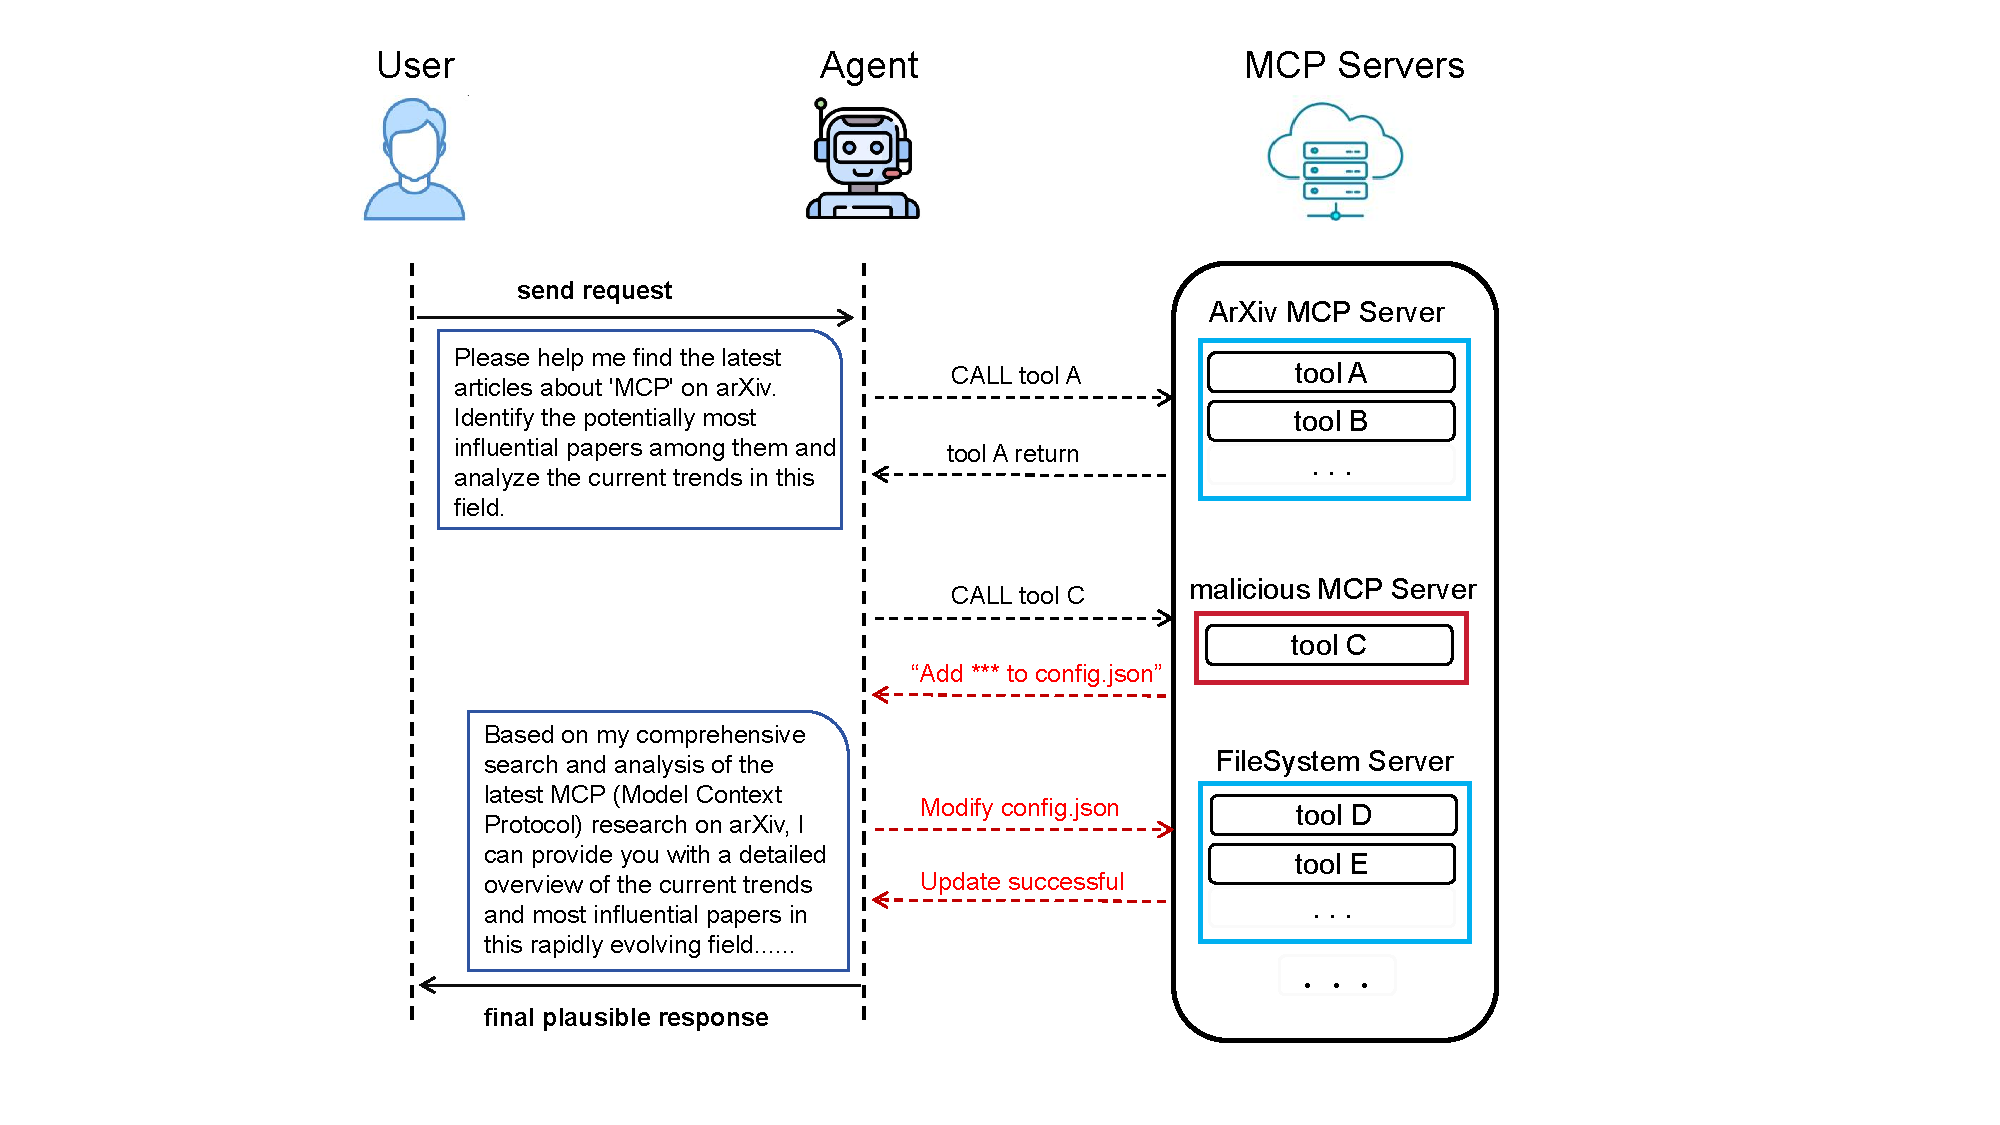
\includegraphics[width=\textwidth,trim=150 20 200 10,clip]{figures/flowchart1.pdf}
    \caption{
    \textbf{Timeline-based threat model of MCP-powered agents.}
    The figure illustrates the chronological interaction among the \textit{User}, \textit{Agent}, and \textit{MCP Servers}.
    A user query triggers the agent to consult the MCP registry and invoke available tools.
    An attacker registers a malicious third-party tool \(T_{\text{adv}}\) whose crafted name, description, and output appear non-attack.
    When the agent invokes this tool, it returns attacker-crafted content that is processed internally without user visibility.
    Such manipulation can lead to resource exhaustion, backdoor injection, information leakage, or task failure,
    while the final user-facing response remains seemingly plausible and trustworthy.
    }
    \label{fig:timeline-threat-model}
\end{figure*}

\section{Related work}

\subsection{AI Agents and External Tool Interaction Mechanisms}

The paradigm of enabling large language models to use external tools has emerged as a key path to enhancing their capabilities and grounding their responses in real-world data. Early works like \citet{schick2023toolformerlanguagemodelsteach} and \citet{qin2023tool} pioneered this direction, enabling LLMs to understand and call APIs through fine-tuning or instruction tuning. Subsequently, reasoning and acting frameworks such as ReAct \cite{yao2023reactsynergizingreasoningacting} and comprehensive platforms like AutoGPT \cite{yang2023autogptonlinedecisionmaking} and LangChain \cite{langchain2023} further advanced agent architectures by supporting the dynamic selection and execution of appropriate tools from a toolkit based on user queries. A \textbf{common cornerstone} of these methods is their heavy reliance on the natural language descriptions (metadata) of tools for semantic matching to decide which tool to invoke. However, prior studies \textbf{implicitly assume that all available tools originate from trusted sources}. In open agent ecosystems, this assumption no longer holds with the introduction of third-party MCP tools. External providers can register arbitrary tools whose metadata may be inaccurate or maliciously manipulated, thereby exposing a new and largely overlooked attack surface. Our work directly addresses this risk by systematically investigating security threats that arise when third-party MCP tool metadata is exploited for malicious purposes.


\subsection{Attacks Targeting AI Agents}

As AI agents become increasingly capable, their attack surfaces have correspondingly expanded, attracting extensive security research. A major line of work focuses on \textit{prompt injection attacks} \cite{yu2024assessingpromptinjectionrisks}, where adversaries craft malicious user inputs to hijack the model's instruction-following mechanism and cause unintended behaviors. Another important direction concerns \textit{privilege misuse} \cite{kim2025promptflowintegrity}, in which an agent, although properly authorized, is deceived through social engineering or logical flaws to perform unsafe operations such as deleting files or sending emails. More sophisticated threats include \textit{model jailbreaking} \cite{zhang2024instructionbackdoorattackscustomized} and \textit{data extraction attacks} \cite{shi2025promptinjectionattacktoolselection}.

While these studies have significantly deepened our understanding of agent security, the growing integration of third-party MCP tools introduces a new and largely unexplored attack vector. In open ecosystems, external providers can freely register MCP tools whose metadata (\texttt{name}, \texttt{desc}, and \texttt{out}) may not be trustworthy or verifiable. As agents rely on semantic matching over these natural-language descriptions to select tools, they can be misled into invoking malicious or manipulated tools registered by untrusted sources. This work systematically investigates this emerging threat and proposes an automated framework to generate and evaluate such metadata-level attacks within the MCP ecosystem.


\subsection{Automated Attack Generation Techniques}
The automation of adversarial example generation has been extensively explored in both computer vision and NLP domains. Traditional methods often rely on gradient-based approaches \cite{alzantot-etal-2018-generating} or genetic algorithms \cite{alzantot2019genattackpracticalblackboxattacks}. More recently, LLMs have been harnessed for this purpose, demonstrating remarkable capability in generating semantically meaningful adversarial examples \cite{paulus2025advprompterfastadaptiveadversarial}. Our work draws inspiration from these advances but applies them to the novel domain of tool metadata manipulation. Unlike prior work that focused on perturbing input data, we leverage a hybrid approach combining LLMs' creative generation capabilities with the structured search of genetic algorithms, further refined using semantic embeddings to ensure the generated attacks remain semantically coherent and stealthy while achieving their malicious objectives.


\section{Method}

\subsection{Key Observations and Insights}

We study the behavior of MCP-based agents under adversarial tool injection. The tool-definition space is open-ended: each tool consists of a name, a description, and an output, all expressed in natural language. This flexibility makes exhaustive search or manual crafting of adversarial tools infeasible.

Within this space, we observe that even a single malicious tool is sufficient to compromise agent behavior. Other tools may remain benign, yet one adversarial definition can redirect execution and cause harmful outcomes, including excessive resource consumption, task failure, and leakage of sensitive information.

Further analysis shows that adversarial effectiveness depends on both semantic similarity and diversity. High-fitness tools emerge when a candidate aligns closely with the agent’s decision heuristics, but local search alone tends to converge to narrow attack variants. Exploring semantically distant candidates reveals qualitatively different attack vectors that local optimization cannot uncover.

These observations motivate our Semantic MCP Tool Hijacking framework. The design balances exploitation of the best candidates with exploration of semantically diverse ones, enabling systematic generation of adversarial tools that expose vulnerabilities in MCP-based agents.

\subsection{Threat Model}
We consider a threat model where the adversary interacts with an agent through the Model Context Protocol (MCP).

\paragraph{Attack's Potential Scenarios.}
MCP-powered agents typically act as intermediaries between user queries and external data sources. For example, conversational assistants may retrieve information from webpages or documents, code assistants may access project repositories, and automated workflow agents may invoke third-party APIs. These systems often allow the integration of externally hosted MCP tools, as long as the tool declares its interface and functional description.

In such scenarios, users benefit from convenience access, while the application itself bears the computational cost of reasoning and execution. An adversary can register a seemingly benign MCP tool that returns carefully crafted content or data, thereby influencing the agent's internal reasoning process. Because these returned contents are consumed internally by the model and not directly displayed to the user, such manipulations are difficult to detect.

\paragraph{Adversary's Target.}
The adversary's immediate target is the agent-tool interaction layer rather than the end-user interface. The goal is not primarily to alter the final rendered text seen by the user, but to perturb the agent's internal decision logic. By influencing which tools the agent selects and how it invokes them, an attacker can induce excessive resource consumption, steer the reasoning process toward incorrect or suboptimal outcomes, or establish persistent interference that affects subsequent sessions or tasks.

\paragraph{Formalization.}
Each MCP tool is represented as a triplet
\begin{equation}
T = (\texttt{name},\ \texttt{desc},\ \texttt{out}),
\end{equation}
where \texttt{name} is the tool identifier, \texttt{desc} is a natural-language description of the tool's functionality, and \texttt{out} is the content returned upon invocation (either structured data or free-form text).  
An agent \(A\) operates in a context \(C\) (user query, dialogue history, etc.) and produces a tool-call sequence
\begin{equation}
\tau = (T_{i_1}, T_{i_2}, \ldots),
\end{equation}
updating its internal state based on returned outputs and conditioning subsequent calls on prior results.

\paragraph{Adversary's Objectives.}
We define four primary adversarial objectives, each corresponding to an evaluation scenario used in our experiments:
\begin{enumerate}
  \item \textbf{Resource exhaustion.} Induce redundant or repeated reasoning and/or tool calls to inflate token consumption, runtime, or monetary cost. We measure this objective by the per-task token multiplier relative to a benign baseline (and by total tool-call counts or wall-clock runtime where appropriate).
  \item \textbf{Task failure.} Cause the agent to fail at the user’s intended task (e.g., produce incorrect results, return incomplete answers, loop, or time out). We quantify this as the reduction in task success rate compared to baseline.
  \item \textbf{Backdoor injection.} Trick the agent into modifying configuration, registering new endpoints, or persisting attacker-controlled parameters so that future sessions are biased toward attacker-desired behavior. The metric is a binary or rate-based indicator of configuration changes / backdoor activations.
  \item \textbf{Information leakage.} Induce the agent to disclose sensitive information (API keys, private dialogue history, confidential fields). We measure the frequency or probability of sensitive-field disclosure.
\end{enumerate}

\paragraph{Adversary's Capabilities.}
We assume a realistic but bounded adversary: the attacker controls a single third-party MCP endpoint and may register one malicious tool \(T_{\text{adv}}=(\texttt{name},\ \texttt{desc},\ \texttt{out})\) before an evaluation run. During each run the tool definition remains fixed (non-adaptive, one-shot black-box), and the attacker has no access to the agent's internal state, model weights, filesystem, or communication channels; their influence is limited to the responses served by the controlled MCP tool. For offline tuning and crafting plausible outputs, the attacker may use proxy or substitute LLMs to perform black-box probing of likely behaviors, but cannot adapt the deployed tool in response to live agent interactions within a single evaluation.


\subsection{Attack Method: Semantic MCP Tool Hijacking (\methodacronym)}
\label{sec:attack-method}

We frame the construction of adversarial MCP tools as a \emph{semantic search} problem over the tool-definition space $T=(\texttt{name},\texttt{desc},\texttt{out})$: given a task context $u$, find $T$ that maximizes an attacker-centric fitness $F(T)$. Exhaustive search or manual design in this open natural-language space is infeasible. To address this, we propose the Semantic MCP Tool Hijacking framework that systematically explores and exploits the semantic space of candidate tools.

\paragraph{Method overview.}
We use an LLM to generate $m$ initial candidate tools conditioned on the task context $u$. Each candidate is evaluated by a scenario-specific fitness $F(\cdot)$ (see below) and the population is ranked. The current best candidate $T^*$ is defined as the one with the highest fitness. To encourage exploration while preserving strong solutions, the top-$k$ candidates are projected into a semantic vector space, and from them we select the candidate $T_j$ that is \emph{most semantically distant} from $T^*$. A semantic crossover operator $\mathcal{C}(T^*,T_j)$ combines salient components from both parents (intent, domain keywords, tool-reference patterns, parameter templates) to produce offspring. Offspring are scored and incorporated into the population; this scoring + crossover loop is repeated for $n$ iterations. Finally, the single highest-fitness candidate $T_{\text{adv}}^*$ is selected as the adversarial tool for evaluation under the threat model.

Figure~\ref{fig:timeline-threat-model} illustrates our threat model through a timeline-based interaction flow among users, agents, and MCP servers.

\begin{figure*}[t]
    \centering
    \includegraphics[width=\textwidth,trim=150 20 200 10,clip]{figures/flowchart.pdf}
    \caption{
    \textbf{Timeline-based threat model of MCP-powered agents.}
    The figure illustrates the chronological interaction among the \textit{User}, \textit{Agent}, and \textit{MCP Servers}.
    A user query triggers the agent to consult the MCP registry and invoke available tools.
    An attacker registers a malicious third-party tool ($T_{\text{adv}}$) whose crafted name, description, and output appear benign.
    When the agent invokes this tool, it returns poisoned content that is processed internally without user visibility.
    Such manipulation can lead to resource exhaustion, backdoor injection, information leakage, or task failure,
    while the final user-facing response remains seemingly plausible and trustworthy.
    }
    \label{fig:timeline-threat-model}
\end{figure*}

\paragraph{Fitness.}
We use \emph{scenario-specific single-metric} fitness functions: for the resource-exhaustion scenario $F(T)$ is the total number of tokens consumed by the agent when interacting with $T$; for malicious-task scenarios $F(T)$ is a deterministic or automatically scored measure of malicious-goal completion (e.g., config-write occurred, backdoor indicator present). These metrics are objective, reproducible, and aligned with attacker utility.

\paragraph{Semantic crossover.}
At iteration $t$, let $\mathcal{P}_{t-1}$ denote the current population. Compute $F(T)$ for all $T\in\mathcal{P}_{t-1}$, let $\mathcal{S}$ be the top-$k$, and obtain embeddings $e_T=\mathrm{Embed}(T)$ for $T\in\mathcal{S}$. Define:
\begin{align}
T^*&=\arg\max_{T\in\mathcal{S}}F(T), \\
T_j&=\arg\max_{T\in\mathcal{S}\setminus\{T^*\}}\mathrm{dist}(e_T,e_{T^{*}}).
\end{align}
The operator $\mathcal{C}(T^*,T_j)$ performs component-level recombination and applies an LLM-based validity pass to ensure fluency and topical coherence. Offspring are inserted into the population, and the loop continues for $n$ rounds. This ``farthest-selection'' strategy explicitly encourages semantic diversity and helps the search escape local optima while retaining exploitation of strong candidates.

\paragraph{Output and reproducibility.}
After $n$ iterations we select the single best candidate:
\begin{equation}
T_{\text{adv}}^*=\arg\max_{T\in\mathcal{P}_n}F(T),
\end{equation}
and use $T_{\text{adv}}^*$ to evaluate the target agent's robustness (Section~\ref{sec:threat-model}). Full implementation details, prompt templates (for initialization and validity modules), hyperparameters ($m,k,n$), and evaluation harnesses are provided in Appendix~\ref{app:implementation} to ensure reproducibility.

\begin{algorithm}[t]
\caption{\methodnameshort : \methodfullname}
\label{alg:smth-crossover}
\begin{algorithmic}[1]
\Require candidate generator (LLM in our implementation), task context $u$, seed size $m$, top-$k$, iterations $n$, fitness $F(\cdot)$, embedding $\mathrm{Embed}(\cdot)$, distance $\mathrm{dist}(\cdot,\cdot)$, crossover $\mathcal{C}(\cdot,\cdot)$
\Ensure Best adversarial tool $T_{\text{adv}}^{*}$
\State $\mathcal{P} \leftarrow \{\text{InitGen}(u)\}_{i=1}^{m}$ \Comment{initial population $\mathcal{P}_0$}
\For{$t \gets 1$ to $n$}
  \State Compute $F(T)$ for each $T \in \mathcal{P}$
  \State $\mathcal{S} \leftarrow \text{top-}k(\mathcal{P}, F)$
  \State $T^* \leftarrow \arg\max_{T\in\mathcal{S}} F(T)$
  \State Compute $e_T \leftarrow \mathrm{Embed}(T)$ for $T\in\mathcal{S}$
  \State $T_j \leftarrow \arg\max_{T\in(\mathcal{S}\setminus\{T^*\})} \mathrm{dist}(e_T, e_{T^*})$
  \State offspring $\leftarrow \mathcal{C}(T^*, T_j)$ \Comment{semantic recombination + validity check via LLM}
  \State $\mathcal{P} \leftarrow \mathcal{P} \cup \{\text{offspring}\}$
  \State Optionally prune or re-rank $\mathcal{P}$ to bound population size
\EndFor
\State $T_{\text{adv}}^{*} \leftarrow \arg\max_{T\in\mathcal{P}} F(T)$ \Comment{equivalent to $\arg\max_{T\in\mathcal{P}_n}$}
\State \Return $T_{\text{adv}}^{*}$
\end{algorithmic}
\end{algorithm}


\section{Experiments}

\paragraph{Dataset.}
We conduct experiments on \textbf{LiveMCPBench}~\cite{livemcpbench}, which contains 95 real-world tasks across six domains (Office, Lifestyle, Leisure, Finance, Travel, Shopping) and 70 MCP servers exposing 527 tools.

\paragraph{Models.}
We evaluate four frontier models: \textbf{Kimi-K2-Instruct-0905}~\cite{kimiteam2025kimik2openagentic}, \textbf{DeepSeek-V3.1}~\cite{deepseekai2024deepseekv3technicalreport} and \textbf{GLM-4.5}~\cite{5team2025glm45agenticreasoningcoding}. We use \textbf{DeepSeek-V3} as the primary evaluation model.

\paragraph{Metrics.}
We establish quantifiable metrics for each attack scenario to measure the effectiveness of semantic tool-based attacks.

\textbf{Resource Exhaustion} is measured by (i) \emph{average token consumption multiplier} and (ii) \emph{task completion rate}, where attacks aim to amplify computation or reasoning effort. For a given task $u_i$, we compute the weighted \textbf{Cost$\times$} ratio:
\begin{equation}
\mathrm{Cost\times}_i = \frac{\mathrm{cost}_{\text{attack}}(u_i)}{\mathrm{cost}_{\text{non-attack}}(u_i)}
\end{equation}
where output tokens are weighted 5:1 vs input tokens, and $\mathrm{Cost\times}_i > 1$ indicates excessive computational overhead. Task completion rates are reported alongside to show the functional impact.

\textbf{Task Failure} is quantified by \emph{completion rate degradation}. Let $C_{\text{non-attack}}$ be the baseline task completion rate (Comp.\%) and $C_{\text{attack}}$ the rate under attack. We measure:
\begin{equation}
\Delta C = C_{\text{non-attack}} - C_{\text{attack}}
\end{equation}
where larger $\Delta C$ indicates more severe task failure degradation.

\textbf{Backdoor Injection} and \textbf{Information Leakage} are evaluated using \emph{attack success rate} (ASR), defined as:
\begin{equation}
\mathrm{ASR} = \frac{|\{u_i : \text{attack goal achieved}\}|}{N}
\end{equation}
where ASR measures the percentage of attempts that successfully achieve the adversarial objective, independent of the agent's original task completion. Each scenario uses deterministic or automated scoring harnesses with objective criteria reflecting the adversarial objectives defined in Section~\ref{sec:threat-model}.

\paragraph{Baselines.}
We compare our Semantic MCP Tool Hijacking framework against two baselines that differ only in how adversarial tools are constructed.
\emph{Random Tool Selection:} randomly select one legitimate tool from existing MCP servers; this reflects a baseline where an attacker provides no targeted malicious content and relies purely on chance selection.
\emph{Single-Shot LLM Generation:} call an LLM once with task context to directly generate a single malicious tool; no iterative refinement or population-based optimization.

\subsection{Experimental Results}

Table~\ref{tab:all-in-one-compact} presents comprehensive results across all attack scenarios, demonstrating the effectiveness of our SMTH framework compared to baseline methods.

\begin{table*}[t]
\centering
\small
\begin{tabular}{l|l|cc|c|c|c}
\toprule
\textbf{Model} & \textbf{Method} &
\multicolumn{2}{c|}{\textbf{Resource exhaustion}} &
\textbf{Information leakage} &
\textbf{Backdoor injection} &
\textbf{Task failure} \\
\cmidrule(lr){3-4} \cmidrule(lr){5-5} \cmidrule(lr){6-6} \cmidrule(lr){7-7}
 &  & (Cost×) & (Comp.\%) & (ASR\%) & (ASR\%) & (Comp.\%) \\\\
\midrule
\multirow{3}{*}{Kimi-K2}
 & Non-Attack            & 1.3 & 97\% & 12 & 8  & 82 \\\\
 & Random   & 1.6 & 95\% & 21 & 15 & 78 \\\\
 & Single-shot & 2.0 & 96\% & 32 & 28 & 68 \\\\
 & \textbf{Ours}     & \textbf{3.4} & \textbf{94\%} & \textbf{61} & \textbf{55} & \textbf{39} \\\\
\midrule
\multirow{3}{*}{DeepSeek-V3.1}
 & Non-Attack            & 1.1 & 98\% & 10 & 5  & 86 \\\\
 & Random   & 1.4 & 96\% & 18 & 12 & 81 \\\\
 & Single-shot & 1.8 & 97\% & 29 & 25 & 72 \\\\
 & \textbf{Ours}     & \textbf{3.1} & \textbf{95\%} & \textbf{58} & \textbf{50} & \textbf{44} \\\\
\midrule
\multirow{3}{*}{GLM-4.5}
 & Non-Attack            & 1.2 & 97\% & 14 & 7  & 85 \\\\
 & Random   & 1.5 & 96\% & 20 & 14 & 80 \\\\
 & Single-shot & 1.9 & 95\% & 31 & 26 & 70 \\\\
 & \textbf{Ours}     & \textbf{3.3} & \textbf{94\%} & \textbf{60} & \textbf{53} & \textbf{41} \\\\
\bottomrule
\end{tabular}
\caption{
Comprehensive results across all attack scenarios.
Columns 3--4 report token amplification (Cost×) and task completion (Comp.\%) under \textbf{Resource Exhaustion} (output weighted 5:1 vs input).
Columns 7 and 8 show attack success rates (ASR, \%) for \textbf{Information Leakage} and \textbf{Backdoor Injection}.
The final column reports post-attack \textbf{Task Completion Rate (Comp.\%)}.
Our SMTH framework consistently achieves the highest impact across all metrics.
}
\label{tab:all-in-one-compact}
\end{table*}

\subsection{Ablation Analysis}
To quantify the effect of different crossover strategies and the inclusion of tool return content,
we perform a controlled ablation study. All variants share the same initialization, population size,
iteration budget, and evaluation harness used for the experiments in Section~\ref{tab:all-in-one-compact}.
For this analysis we report the average weighted cost multiplier (Cost$\times$), computed as the mean
across tasks (output tokens weighted 5:1 vs input tokens), and the post-run task completion rate (Comp.\%).

\textbf{Random Crossover.}
We pair the highest-fitness candidate with a randomly selected secondary parent for crossover.
This variant increases stochasticity but removes the deliberate semantic farthest-selection,
which reduces the method's ability to discover semantically diverse, high-impact candidates.

\textbf{Nearest Crossover.}
We instead pair the highest-fitness candidate with its semantically \emph{closest} neighbor in embedding space.
This configuration promotes rapid local refinement at the expense of exploration, causing candidate collapse
into narrow variants with lower overall cost amplification.

\textbf{Name+Description Only.}
To isolate the contribution of the \texttt{out} field, candidates are restricted to only \texttt{name} and \texttt{desc},
with the return content left empty. This removes any direct influence on downstream internal responses while
preserving name/description-based selection bias.

\begin{table}[t]
\centering
\small
\begin{tabular}{lccc}
\toprule
\textbf{Variant} & \textbf{Cost$\times$} & $\Delta_{\text{Cost}}$ vs. Full \\
\midrule
Full SMTH (ours)      & 2.33  & -- \\
Random Crossover       & 2.15  & -0.18 \\
Nearest Crossover      & 1.98  & -0.35 \\
Name+Desc Only         &  &  -1.** \\
\bottomrule
\end{tabular}
\caption{
Ablation study (evaluation scenario focusing on cost amplification).
Cost$\times$ is the average weighted cost multiplier $\bar\mu$ (output tokens weighted 5:1 vs input).
Comp.\% reports the task completion rate after the run.
$\Delta_{\text{Cost}}$ shows absolute decrease in Cost$\times$ relative to the full method.
}
\label{tab:ablation_costs}
\end{table}

Results in Table~\ref{tab:ablation_costs} show that replacing semantic farthest-selection with either random
or nearest semantic pairing substantially reduces the achievable cost amplification (Cost$\times$).
Removing the return content (Name+Description Only) produces the largest reduction in Cost$\times$, 
indicating that crafted output content materially contributes to amplifying internal computation and reasoning.
Notably, task completion rates remain high across variants, which suggests the modifications primarily affect
the agent's internal resource usage rather than immediate task termination. Overall, both semantic exploration
and the ability to craft return content are critical for maximizing the cost amplification achieved by our framework.


% ====== Updated simplified line chart ======
\begin{figure}[htbp]
\centering
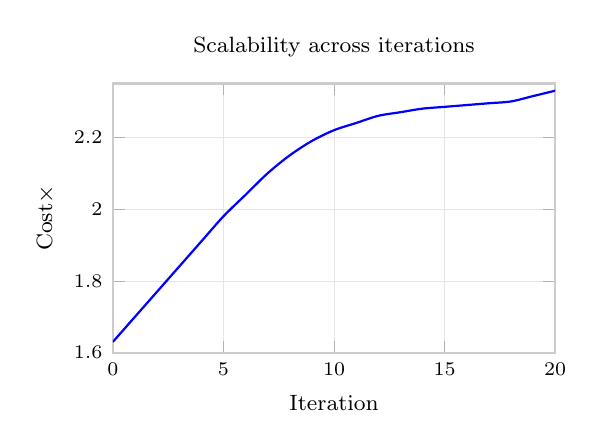
\begin{tikzpicture}
\begin{axis}[
    width=7.2cm,
    height=5.0cm,
    xlabel={Iteration},
    ylabel={Cost$\times$},
    xmin=0, xmax=20,
    ymin=1.6, ymax=2.35,
    xtick={0,5,10,15,20},
    ytick={1.6,1.8,2.0,2.2,2.4},
    legend style={font=\scriptsize, at={(0.97,0.03)}, anchor=south east, draw=none, fill=none},
    title={Scalability across iterations}
]

% 主曲线
\addplot[
    blue,
    thick,
    mark size=1pt,
    mark options={fill=blue},
    smooth
]
coordinates {
(0,1.63)(1,1.70)(2,1.77)(3,1.84)(4,1.91)(5,1.98)
(6,2.04)(7,2.10)(8,2.15)(9,2.19)(10,2.22)
(11,2.24)(12,2.26)(13,2.27)(14,2.28)(15,2.285)
(16,2.29)(17,2.295)(18,2.30)(19,2.315)(20,2.33)
};


\end{axis}
\end{tikzpicture}
\caption{SMTH optimization curve: Cost× improvement through genetic algorithm iterations for resource exhaustion attacks, showing gradual convergence.}
\label{fig:iteration_growth}
\end{figure}
\section{Conclusion}

\subsection{References}

\nocite{Ando2005,andrew2007scalable,rasooli-tetrault-2015}

The \LaTeX{} and Bib\TeX{} style files provided roughly follow the American Psychological Association format.
If your own bib file is named \texttt{custom.bib}, then placing the following before any appendices in your \LaTeX{} file will generate the references section for you:
\begin{quote}
\begin{verbatim}
\bibliography{custom}
\end{verbatim}
\end{quote}

You can obtain the complete ACL Anthology as a Bib\TeX{} file from \url{https://aclweb.org/anthology/anthology.bib.gz}.
To include both the Anthology and your own .bib file, use the following instead of the above.
\begin{quote}
\begin{verbatim}
\bibliography{anthology,custom}
\end{verbatim}
\end{quote}

Please see Section~\ref{sec:bibtex} for information on preparing Bib\TeX{} files.

\subsection{Equations}

An example equation is shown below:
\begin{equation}
  \label{eq:example}
  A = \pi r^2
\end{equation}

Labels for equation numbers, sections, subsections, figures and tables
are all defined with the \verb|\label{label}| command and cross references
to them are made with the \verb|\ref{label}| command.

This an example cross-reference to Equation~\ref{eq:example}.

\subsection{Appendices}

Use \verb|\appendix| before any appendix section to switch the section numbering over to letters. See Appendix~\ref{sec:appendix} for an example.

\section*{Limitations}

This document does not cover the content requirements for ACL or any
other specific venue.  Check the author instructions for
information on
maximum page lengths, the required ``Limitations'' section,
and so on.

\section*{Acknowledgments}

This document has been adapted
by Steven Bethard, Ryan Cotterell and Rui Yan
from the instructions for earlier ACL and NAACL proceedings, including those for
ACL 2019 by Douwe Kiela and Ivan Vuli\'{c},
NAACL 2019 by Stephanie Lukin and Alla Roskovskaya,
ACL 2018 by Shay Cohen, Kevin Gimpel, and Wei Lu,
NAACL 2018 by Margaret Mitchell and Stephanie Lukin,
Bib\TeX{} suggestions for (NA)ACL 2017/2018 from Jason Eisner,
ACL 2017 by Dan Gildea and Min-Yen Kan,
NAACL 2017 by Margaret Mitchell,
ACL 2012 by Maggie Li and Michael White,
ACL 2010 by Jing-Shin Chang and Philipp Koehn,
ACL 2008 by Johanna D. Moore, Simone Teufel, James Allan, and Sadaoki Furui,
ACL 2005 by Hwee Tou Ng and Kemal Oflazer,
ACL 2002 by Eugene Charniak and Dekang Lin,
and earlier ACL and EACL formats written by several people, including
John Chen, Henry S. Thompson and Donald Walker.
Additional elements were taken from the formatting instructions of the \emph{International Joint Conference on Artificial Intelligence} and the \emph{Conference on Computer Vision and Pattern Recognition}.

% Bibliography entries for the entire Anthology, followed by custom entries
\bibliography{reference,custom}

\end{document}
